\documentclass[10pt,a4paper]{article}
\usepackage[latin1]{inputenc}
\usepackage{amsmath}
\usepackage{amsfonts}
\usepackage{amssymb}
\usepackage{graphicx}
\usepackage[width=16.00cm, height=22.00cm]{geometry}

\usepackage{siunitx}

\usepackage[acronym,translate=false]{glossaries}
\usepackage[backend=biber,style=bwl-FU,uniquename=false,maxbibnames=99]{biblatex}
\addbibresource{bibrefs.bib}

\usepackage{setspace}
%\singlespacing
%\onehalfspacing
\doublespacing
%\setstretch{1.1


\usepackage{chngcntr}
\counterwithin{figure}{section}
\counterwithin{equation}{section}

%\title{The Importance of Eddy-Topographic Interactions for Arctic
%	Ocean Dynamics and Steps Towards Improving Climate Models}
%\author{Mark Edward Forshaw\\ Department of Physics\\
%University of Oxford\\ E-mail: \url{forshaw@atm.ox.ac.uk}}


\newacronym{amoc}{AMOC}{Antarctic~Meridional~Overturning~Circulation}
\newacronym{bas}{BAS}{British~Antarctic~Survey}
\newacronym{arp}{ARP}{Arctic~Research~Program}
\newacronym{ipy}{IPY}{International~Polar~Year}
\newacronym{awl}{AWL}{Atlantic~Water~Layer}
\newacronym{aomip}{AOMIP}{Arctic~Ocean~Model~Inter--comparison~Project}
\newacronym{pv}{PV}{potential vorticity}
\newacronym{gcm}{GCM}{Global~Climate~Model}
\newacronym{bso}{BSO}{Barents~Sea~Opening}
\newacronym{gm}{GM}{Gent~and~Mcwilliams~Parameterisation}

\newcommand*\mean[1]{\overline{#1}}
\newcommand*\res[1]{{#1}^{\prime}}
\newcommand*\thkmean[1]{\overline{#1}}
\newcommand*\thkres[1]{{#1}^{\prime}}
\newcommand*\nthkmean[1]{\left\langle{#1}\right\rangle}
\newcommand*\nthkres[1]{{#1}^{\#}}
\newcommand*\spec[1]{\mathring{#1}}

\nocite{cushman2011introduction}
\nocite{vallis2006atmospheric}

\title{Draft}


\begin{document}

\maketitle


\section{Introduction}

\glsresetall

\subsection{Arctic Ocean}
\label{arcticocean}


Despite its small size (only $3\%$ of the Earth's surface), the Arctic
Ocean is a disproportionately important part of the global ocean and has the potential
to affect the world's climate in major ways. Located above
$70\,^{\circ}{\rm N}$, the Arctic is characterised by its seasonally
varying ice cap. This ice cap, along with its counterpart at the South
Pole, is a major contribution to the planet's albedo as well as being
a large reservoir for freshwater. The Arctic Ocean is a key component
in how the polar ice cap interacts with the climate and, in turn, how
the climate affects the ice cap. 
The Ocean itself is a highly stable body of water with strong stratification, 
which means that the water column can be divided into advective water masses.
The Arctic Ocean is commonly divided into four different layers (Figure~\ref{fig:amap}):
The polar mixed layer, which is a well mixed layer in
contact with the atmosphere and surface ice; the halocline, which acts as
reservoir of fresh water and penetrates to around ${\sim}200\,{\rm m}$; the \gls{awl},
which is body of warm salty water which originates from the North Atlantic and Nordic 
Sea via Fram Strait and typically sits at around ${\sim}400\,{\rm m}$ deep; and finally, 
the Arctc Deep Water, defined by the water masses that aren't
able to communicate freely with the global ocean due to being trapped by the Arctic basin's walls.



\begin{figure}
	\centering
	\includegraphics[width=\linewidth]{amap}
	\caption[\cite{wilson1998amap}]{  A schematic representation of the four-layer structure of the Arctic Ocean, with the Mixed Layer and Halocline
		above the Atlantic Water and Arctic Deep Water (\cite{aagaard1989role}). 
		The residence time for the different water masses are also shown (\cite{bonisch1995deep}). \cite{wilson1998amap}.}
	\label{fig:amap}
\end{figure}

Because of the strong stratification, the forcing from the ocean surface 
struggles to penetrate deep into the ocean; and so whether forced directly by wind 
or by sea ice stress, the circulation
directly forced from the surface is contained within the polar mixed layer 
and halocline in the upper ${\sim}200\,{\rm m}$ of the Arctic Ocean. 
This surface circulation has been well documented by observations
from cruises and moorings  dropped  from  the  ice  shelf  or  deployed  on 
the  shallower  continental  shelves (\cite{gerdes1997large}, \cite{jones2001circulation}). On the other hand, it's a very different
story for the circulation in the \gls{awl} and lower layers (Figure~\ref{fig:Proshutinsky2005Circulation}). Observations made
inside the Ocean's basins rarely are able to profile the structure  and
circulation  below 500m  although much progress has been made here in the
past decade. This lack of observations means that  we  still only have  a  sense  of  the circulation 
of the \gls{awl} and the Deep  Waters.  The  observations  we  do 
have  infer stable cyclonic  rim  currents about each of the basins in the
\gls{awl} and it is believed that this trend extends through the Deep Water to the 
ocean floor.  Because of the highly stratified nature of the halocline, the surface forcing 
is likely to have little effect on the deeper ocean, which leaves the other 
two possibilities as the determining features.


\begin{figure}
	\centering
	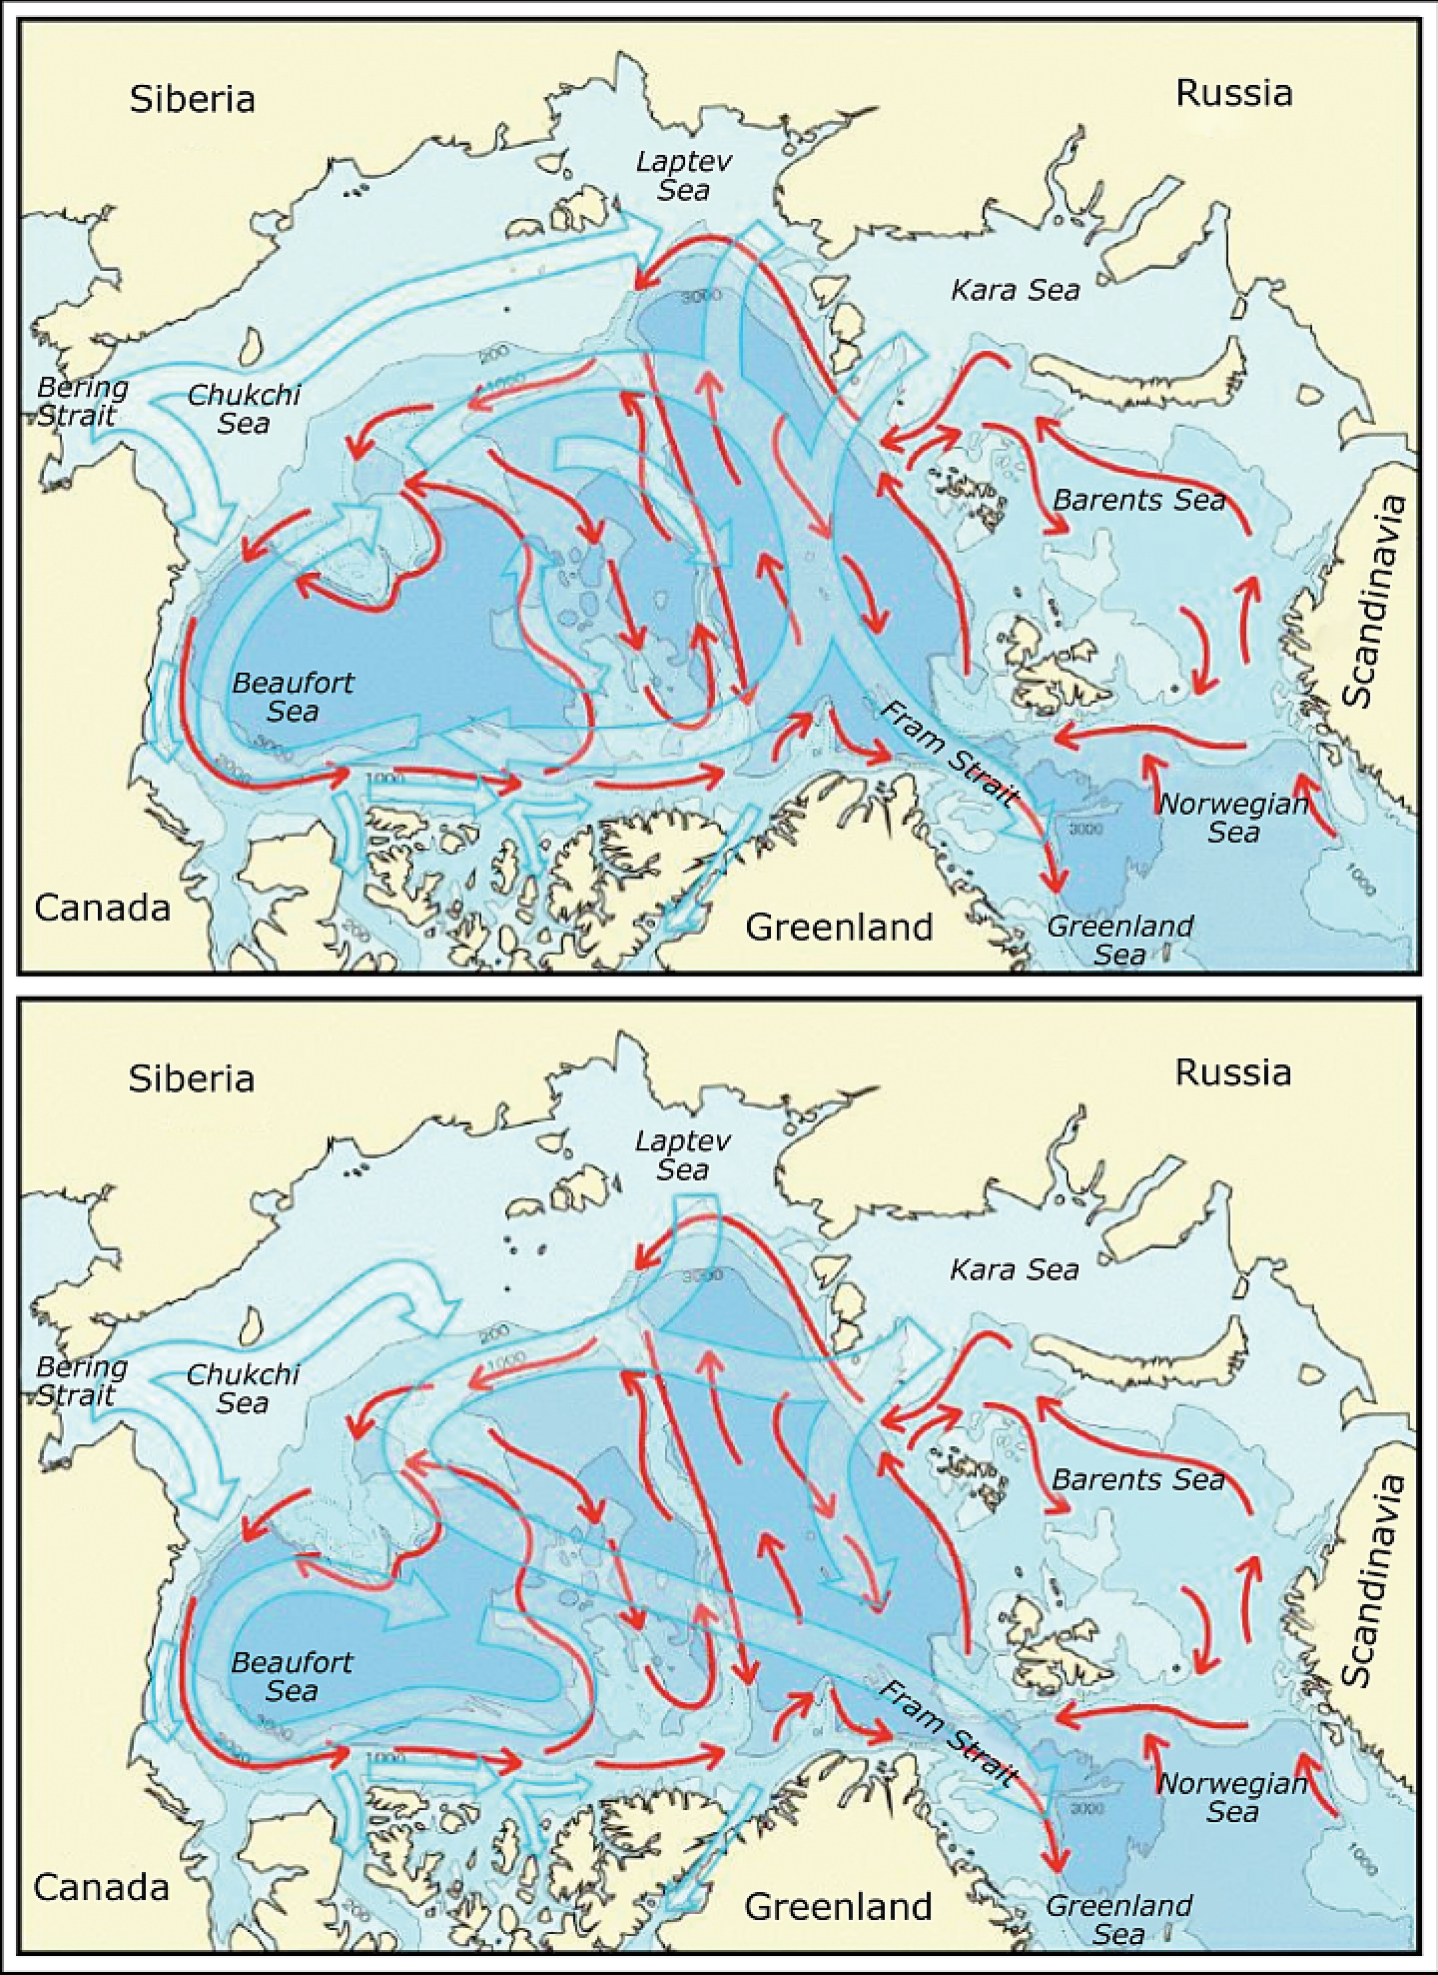
\includegraphics[width=0.9\linewidth]{Proshutinsky2005Circulation}
	\caption[\cite{proshutinsky2005arctic}]{ Two freshwater layer regimes (light 
		blue arrows) overlaying the cyclonic rim currents of the \gls{awl} (red arrows).
		Whilst the Freshwater regimes are vastly different from each other, the
		\gls{awl} is unaffected and remains persistently cyclonic.
		Topography is represented in the background running from 
		shallow water (light blue) to deep water (dark blue).  \cite{proshutinsky2005arctic}.}
	\label{fig:Proshutinsky2005Circulation}
\end{figure}

There has been much discussion
into how the fluxes in and out of the Arctic could influence the circulation,
for example, by a forcing a balance of \gls{pv} within the region by
the fluxes of \gls{pv} though the boundaries. \cite{yang2005arctic} demonstrates how,
in an idealised barotropic model of a basin, controlling the flux 
of \gls{pv} through inflows and outflows
at the boundary, the circulation in the basin could be switched between cyclonic and
anti-cyclonic circulations (Figure~\ref{fig:Yang2005}). This principle suggests
that the persistent cyclonic nature of the \gls{awl} implies that there is a 
net influx of \gls{pv} via the Arctic Gateways. Fortunately, permanent moorings 
covering the majority of the ocean gateways into the Arctic~Ocean have built
up a detailed picture of the transport in and out of the Arctic Ocean 
(\cite{tsubouchi2012arctic}, Figure~\ref{fig:Tsubouchi2012Transport}). The net flux of \gls{pv} is then estimated by summing the distribution of \gls{pv}; given by $ \Pi_{i} = fQ_{i}/H_{i}$,
where $Q_{i}$ is the volume transport and $H_i$ the depth, for location $i$. 
Whilst there is a tendency for total to infer a positive influx of \gls{pv}, the
results are not convincing; \cite{munchow2006observational} shows that by including the
Canadian Archipelago in the \cite{yang2005arctic} calculation the flux can be negated whilst
\cite{tsubouchi2012arctic} demonstrates large variations of transport from the mean over time.
These factors, especially the large variability, make it unconvincing that its the \gls{pv}
 transport, or in fact any properties of the gateway fluxes, that determines the 
cyclonic nature of the \gls{awl}.
Hence, the deep water circulation in the Arctic Ocean is more likely determined by 
internal processes, which are poor understood, especially in an Ocean with such sparse observations.

\begin{figure}
	\centering
	\includegraphics[width=\linewidth]{Yang2005}
	\caption[\cite{yang2005arctic}]{ The circulation of two simple barotropic
		models. The background colour is the model bathymetry. The left plot has
		a net influx of \gls{pv} (the inflow is shallower than the outflow) 
		and a cyclonic circulation whilst the right plot has net outflux of  \gls{pv} 
		and an anti-cyclonic circulation. \cite{yang2005arctic}.}
	\label{fig:Yang2005}
\end{figure}


\begin{figure}
	\centering
	\includegraphics[width=\linewidth]{Tsubouchi2012Transport}
	\caption[Adapted from \cite{tsubouchi2012arctic}]{Velocity
		sections (${\rm cm} \, {\rm s}^{-1}$) from Arctic gateway mooring arrays;
		Demonstrates the pathways through the gateways, from which transport 
		in to the Arctic can be calculated.
		Bold black lines show certain isopycnals, and the red (blue) colors show inflow
		into (outflow from) the Arctic.  Adapted from \cite{tsubouchi2012arctic}.}
	\label{fig:Tsubouchi2012Transport}
\end{figure}

A likely candidate for generating a cyclonic circulation in the Northern hemisphere is
geostrophic turbulence. A number of studies have demonstrated how, in an eddying system, 
sloping topography can generate along-topography flows (\cite{treguier1989topographically}, \cite{adcock2000interactions}, \cite{nost2008asymmetry}). Hence, in the absence of stronger
forcing, this effect is likely to become the dominant feature. An obvious question that then
comes to mind is how turbulent is the Arctic Ocean? Over recent years a large amount  of 
effort has been made to observe and catalogue eddies in the Arctic
(\cite{zhao2014characterizing}) and has demonstrated their prevalence in the Arctic Ocean.
Whilst these studies have frequently been focused on the halocline and the surface dynamics
there is good reason to believe that eddies also penetrate deep into the Arctic 
(Figure~\ref{fig:Woodgate2001Mooring}, \cite{woodgate2001arctic}).



\begin{figure}
	\centering
	\includegraphics[width=\linewidth]{Woodgate2001Mooring}
	\caption[Adapted from \cite{woodgate2001arctic}]{A Velocity Stickplot 
		from a year-long mooring at \ang{78;30.8;} N, \ang{133;57.7;} E, west of the Lomonosov Ridge.  The plot shows a huge amount of variability over time, with many
		features being persistent throughout the water column. Adapted from \cite{woodgate2001arctic}.}
	\label{fig:Woodgate2001Mooring}
\end{figure}

\subsection{Mean-Eddy Interaction Theory}

\label{meaneddyinteractiontheory}

 Obviously, whilst observations play a vital role in understanding the Arctic
 Ocean and its role in the global ocean, it is limited by the sparsely available
 observations that only usefully reach back a handful of decades into the past.
 To be able to test possible scenarios and make future predictions it is vital
 that we have reliable simulations of the Arctic Ocean (\cite{proshutinsky2008toward});
 however, due to limitations
 in modern computing power and poor understanding of the unresolved processes 
 in the ocean this is, more often than not, far from reality.
 Due to these computational limits a practical \gls{gcm} is 
 limited to a  resolution of the order of tens of kilometres. This means that with a 
 resolution  cut off at around $10 \textendash 100 \, \rm km$, 
 \glspl{gcm} are unable to fully resolve a large portion of the mesoscale turbulence that is
 observed in the physical ocean.
 By attempting  to understand the physics behind these unresolved processes 
 and developing parameterisations that mimic their effect on the resolved ocean
 the value of computational models can be improved without dramatically increasing the
 computing power required.  
 
 The turbulent, chaotic nature of the ocean is caused by the non-linearity of its 
 governing equations. Because of this,  the discretisation of the equations generates cross-correlation, or eddy, terms when applying the 
 averaging operator,
 \begin{equation}
 \mean{\phi\psi} = \mean{\phi}\,\mean{\psi} + 
 \mean{\res{\psi}\res{\psi}},
 \label{non-lin average}
 \end{equation}
 where the ${\mean{\phi}}$ is the average of the variable ${\phi}$, used in
 the discretisation and satisfying
 the expected properties of an averaging operator, and the prime denotes the residual, ${\phi^{\prime} = \phi - \mean{\phi}}$.
 The discretised system has no knowledge of the residual terms and hence
 the contributions to the full system by these eddy terms are
 ignored in the discretised system. It is, therefore, this ``sub-grid scale process"
 that is missing from the model dynamics and so it is common practise to try and
 `close' the system by including a parameterisation of the eddy
 term in place of the term itself, which is usually dependent on the averaged 
 variables and some physical assumptions.
 
 The earliest ocean models (\cite{bryan1969numerical}) had vertical $z$-coordinate, or depth-coordinates, with simple horizontal and vertical Laplacian diffusion to act as 
 the closure. Whether these terms are interpreted as a parameterisation for the effects
 of unresolved turbulence or simply as a numerical tool to avoid noise at 
 the grid scale, the viscosity parameter is tuned such that the turbulent energy cascade is 
 dissipated at the grid scale whilst still allowing as active dynamics as possible. 
 Assuming modern day computing power this implies a horizontal viscosity of around 
 $10^{5} - 10^{7} \rm Pa \cdot s$, a viscosity more suited to peanut butter than 
 a the ocean. A second problem with having such a strong horizontal diffusion is
 that it diffuses or mixes tracers horizontally, when applied as
 an eddy parameterisation for tracer mixing. It has long been understood that tracers 
 mix much more along isopycnal surfaces than across them (\cite{iselin1939influence}, \cite{montgomery1940present}), which is a property which allowed for the definition of
 distinct water masses in the global ocean (for example, \cite{emery1986global}).
  Hence, with an excessive horizontal diffusion
 of tracers ocean models are able to break up water masses much quick than
 is observed in the physical ocean creating, for example, the "Veronis Effect" (\cite{veronis1975role}).
 Hence, a more physically appropriate eddy parameterisation 
 is needed;
  and so, in a way that seems obvious today, eddies need to be
   parameterised in 
 such a way that their effect acts along isopycnal surfaces. 
 The effort to do this in the 80's and early 90's gave birth
 to what is known as the \gls{gm}, first introduced in \cite{gent1990}.
 
 So what is the \gls{gm} parameterisation? Since mixing occurs primarily
 along isopycnal surfaces it make sense to have this discussion in
 isopycnal coordinates, that is in the coordinate space $(x,y,\rho)$,
  where density, $\rho$, has replaced depth, $z$, as the vertical
  coordinate. Whilst the rigorous exploration of this coordinate system
  will be discussed in detail later in this section, for our current purposes 
  it is enough to say that this coordinate system produces an equation
  for isopycnal "thickness",
  \begin{equation}
  \label{cont}
  \frac{\partial z_{\rho}}{\partial t} + \boldsymbol{\nabla}\cdot\left(z_{\rho}\boldsymbol{u}\right) = 0,
  \end{equation}
  where $z_{\rho} = \frac{\partial z}{\partial \rho}$ is defined as the
   isopycnal thickness and $\boldsymbol{u}$ is the horizontal fluid
   velocity. Since it is non-linear, when this equation is discretised
   it produces an eddy covariance term as demonstrated by equation
   \ref{non-lin average}; the averaged equation can be written as
     \begin{equation}
     \frac{\partial \mean{z_{\rho}}}{\partial t} + \boldsymbol{\nabla}\cdot\left(\mean{z_{\rho}} \, \mean{\boldsymbol{u}}\right) = - \boldsymbol{\nabla}\cdot\left(\mean{\res{z_{\rho}} \res{\boldsymbol{u}}}\right).
     \label{meancont}
     \end{equation}
   The eddies should therefore be parameterised by some representation
   of $\mean{\res{z_{\rho}} \res{\boldsymbol{u}}}$, say $\boldsymbol{F}$,
   so that the thickness equation becomes
     \begin{equation}
     \frac{\partial z_{\rho}}{\partial t} + \boldsymbol{\nabla}\cdot\left(z_{\rho}\boldsymbol{u}\right) + \boldsymbol{\nabla}\cdot\boldsymbol{F} = 0,
     \label{thicknessgeneralparam}
     \end{equation}
    where the bars have been dropped for convenience. It can also 
    be noted that by defining $\hat{\boldsymbol{u}} = \boldsymbol{F}/z_{\rho}$ the above equation can be interpreted as
    the isopycnal thickness
    being advected by the mean horizontal velocity, $\boldsymbol{u}$, 
    plus an eddy induced
    `bolus velocity', $\hat{\boldsymbol{u}}$. \cite{gent1990} then goes one
    step further and proposes that eddies act to homogenise each
    isopyncal layer via baroclinic instability, hence the 
    \gls{gm} parameterisation is given by $\boldsymbol{F} = - \left(\kappa
    \boldsymbol{\nabla} z \right)_{\rho}$, where $\kappa$ can both be
     spatially and temporally varying parameter. Combining this with equation \ref{thicknessgeneralparam} we have
          \begin{equation}
          \frac{\partial z_{\rho}}{\partial t} + \boldsymbol{\nabla}\cdot\left(z_{\rho}\boldsymbol{u}\right) = \boldsymbol{\nabla}\cdot\left(\kappa
              \boldsymbol{\nabla} z \right)_{\rho} .
              \label{contgm}
          \end{equation}
    Similarly, for a tracer, say $\tau$, we can write an equation
    describing it's transport,
            \begin{equation}
              \frac{\partial \tau}{\partial t} + \boldsymbol{u}\cdot\boldsymbol{\nabla}\tau = \boldsymbol{\nabla}\tau\cdot
              \left(\kappa \boldsymbol{\nabla} z \right)_{\rho}/z_{\rho} .
            \end{equation}
            
    There are a few properties of this parameterisation that can be 
    noted to help describe its overall effect of its implementation in
    ocean models. Firstly, by writing $\boldsymbol{u}^{\star} = \boldsymbol{u} -
    \left(\kappa \boldsymbol{\nabla} z \right)_{\rho}/z_{\rho}$ we 
    simply have that $\frac{\partial z_{\rho}}{\partial t} + \boldsymbol{\nabla}\cdot\left(z_{\rho}\boldsymbol{u}^{\star}\right) = 0$ and $\frac{\partial \tau}{\partial t} + \boldsymbol{u}^{\star}\cdot\boldsymbol{\nabla}\tau = 0$ indicating
    that the tracer $\tau$ is effectively advected by a transport velocity, 
     $\boldsymbol{u}^{\star}$. Secondly, an important 
    question is how does \gls{gm} change the energy of the system. 
    The right hand side of equation \ref{contgm} adds 
    $\phi \boldsymbol{\nabla}\cdot\left(\kappa
                  \boldsymbol{\nabla} z \right)_{\rho} 
                  = \boldsymbol{\nabla}\cdot\left(\phi\kappa
                       \boldsymbol{\nabla} z \right)_{\rho} 
                  -\left(\kappa
              \boldsymbol{\nabla}\phi\cdot \boldsymbol{\nabla} z \right)_{\rho} 
                                -\left(\kappa g
                            \boldsymbol{\nabla}z\cdot \boldsymbol{\nabla} z \right)/{\rho_{0}} 
                $ to the energy tendency. Integrating over an entire domain
                eliminates the first two terms leaving the final term
                as a positive definite sink of energy. These two 
                properties characterise \gls{gm}; the parameterisation
                acts along isopycnal surfaces to flatten isopycnal 
                surfaces whilst dissipating potential energy.
                
        The dissipative nature of \gls{gm} is both an strength and a
         weakness. \gls{gm} is incapable of introducing spurious energy,
         which allows it to be very robust and stable meaning it can be implemented 
         into a \gls{gcm} with little tuning. However, it is also understood that
         ocean turbulence is not purely dissipative.
          \cite{adcock2000interactions} concisely demonstrated that
         in an idealised model, with no external forcing other
         than an initial eddy field, will develop a persistent along
         topography flow and the isopycnals will dome slightly above topography.
          \cite{nost2008asymmetry} showed that these
         flows develop asymmetrically, such that the flow is 
         predominantly cyclonic in
         a basin in the northern hemisphere. For this to occur 
         when the eddy field is unresolved there must be an 
         injection of energy into the system representing the 
         inverse cascade of energy from the eddy scales to the large scale.
         However, this is prohibited by the purely dissipative \gls{gm}
         and so a different parameterisation is required to mimic this
         effect.
         
         To proceed one might wonder what makes the continuity equation
         so special, in truth there is a number of non-linearities that
         crop up when examining the full state equations. Take, for example, the
         absolute vorticity, which can be written in the same form as the continuity equation, i.e.
           \begin{equation}
           \frac{\partial \omega}{\partial t} + \boldsymbol{\nabla}\cdot\left(\omega\boldsymbol{u}\right) = 0,
           \label{vort}
           \end{equation}
           where $\omega=f+\xi$ is the absolute vorticity and
           $\xi = \boldsymbol{k} \cdot\left( \boldsymbol{\nabla}\wedge \boldsymbol{u}\right)$ is the relative vorticity. 
           By applying an average operator to Equation \ref{vort}, we have the same averaged equation as Equation \ref{meancont} but for the mean absolute vorticity, $\mean{\omega}$,
                \begin{equation}
                \frac{\partial \mean{\omega}}{\partial t} + \boldsymbol{\nabla}\cdot\left(\mean{\omega} \, \mean{\boldsymbol{u}}\right) = - \boldsymbol{\nabla}\cdot\left(\mean{\res{\omega} \res{\boldsymbol{u}}}\right),
                \end{equation}
                which to close in a numerical model requires the
                right hand side, $- \boldsymbol{\nabla}\cdot\left(\mean{\res{\omega} \res{\boldsymbol{u}}}\right)$, to be parameterised.
                \cite{greatbatch1998exploring} makes the observation
                here that the mechanism this equation is describing 
                is much clearer if we note the following; if we take
                $\mean{q}$ to be the thickness weighted mean of $q$, i.e.
                $\mean{q}=\mean{z_{\rho}q}/\mean{z}_{\rho}$, then 
                $\mean{\omega}=\mean{q}\,\mean{z}_{\rho}$ and $\res{\omega}=\mean{z}_{\rho}\res{q}+\mean{q}\res{z}_{\rho}$. By 
                combining this with Equation \ref{meancont} we gain a conservative equation 
                for \gls{pv}, 
                \begin{equation}
                \frac{\partial \left(\mean{z}_{\rho} \mean{q}\right)}{\partial t} +
                 \boldsymbol{\nabla}\cdot\left(\mean{z}_{\rho}\,\mean{q}\,\mean{\boldsymbol{u}}+\mean{q}\mean{\res{z}_{\rho} \res{\boldsymbol{u}}}\right)
                 = - \boldsymbol{\nabla}\cdot\left(\mean{z}_{\rho}\,\mean{\res{q} \res{\boldsymbol{u}}}\right) .
                 \label{meanpveq}
                \end{equation}
                This being the form of \gls{pv}, which leads to the impermeability theorems
                of \cite{haynes1987evolution} and \cite{haynes1990conservation}.
                
                Now, by making the same assumption that was made for isopycnal thickness in 
                \gls{gm} for \gls{pv}, that ocean eddies mix PV along isopycnals and not
                across them, equation \ref{meanpveq} becomes
                \begin{equation}
                \frac{\partial \left(\mean{z}_{\rho} \mean{q}\right)}{\partial t} +
                \boldsymbol{\nabla}\cdot\left(\mean{z}_{\rho}\,\mean{q}\,\mean{\boldsymbol{u}}+\mean{q}\mean{\res{z}_{\rho} \res{\boldsymbol{u}}}\right)
                = \boldsymbol{\nabla}\cdot\left(\kappa \mean{z}_{\rho}\,\boldsymbol{\nabla}\mean{q}\right) ,
                \label{parammeanpveq}
                \end{equation}
                where we've used the small slope approximation, demonstrated in \cite{gent1990}. By using Equations \ref{meancont} and \ref{parammeanpveq} we have exactly the equation for an arbitrary tracer given in Equation 6 of \cite{gent1995parameterizing},
                \begin{equation}
                \frac{D^\star \mean{q}}{D t}\equiv\frac{\partial \mean{q}}{\partial t} + \boldsymbol{u}^\star\cdot\boldsymbol{\nabla}\mean{q} = \boldsymbol{\nabla}\cdot
                \left(\kappa \mean{z}_{\rho}\boldsymbol{\nabla} \mean{q} \right)/\mean{z}_{\rho} ,
                \label{pvclosure}
                \end{equation}
                applied to the mean \gls{pv}, which is advected by the transport velocity $\boldsymbol{u}^\star$ and diffused along isopycnal surfaces. This is now
                the \gls{pv} closure first proposed in \cite{greatbatch1998exploring}.
                
                Equation \ref{pvclosure} represents the interaction of eddies as the
                down-gradient diffusion of \gls{pv}; and hence suggests that eddies
                act to homogenise \gls{pv}. Since \gls{pv} can be approximately written
                as $q=f/\sigma$ for small relative vorticity, the parametrisation acts  to homogenise isopycnal thickness. In the case 
                where there is no topography this is identical to the flattening of isopycnals.
                However, in the presence of topography homogenised isopycnal thickness
                causes the isopycnals to mimic the shape of the topography and hence 
                rise over topography. However, to allow this to happen freely
                clearly violates energy conservation, as demonstrated schematically in 
                Figure \ref{fig:Colddoming}. In reality, the ocean attempts to 
                homogenise \gls{pv} but only so far as it can with the available energy;
                the result is the slight ``cold doming" above topography as observed in
                \cite{adcock2000interactions}. 
                
                It isn't all bad news though. Whilst, unlike \gls{gm}, the downgradient
                dissipation of \gls{pv} capable of introducing spurious energy, it does
                control another important quantity: Enstrophy. By multiplying through 
                by $\mean{z}_{\rho} \mean{q}$, Equation \ref{pvclosure} becomes 
                \begin{equation}
                \frac{\partial  }{\partial t}\left(\frac{1}{2}z_{\rho}q^{2}\right) + \boldsymbol{\nabla}\cdot\left(z_{\rho}q\boldsymbol{u}^\star-\kappa z_{\rho}q\boldsymbol{\nabla} q
                \right)=-\kappa z_\rho \boldsymbol{\nabla}q\cdot\boldsymbol{\nabla}q
                \end{equation}
                where the bars have been dropped for convenience.
                Integrating over the entire domain eliminates the divergent term
                leaving just a positive definite dissipation.
                Hence, in the same way that \gls{gm} dissipates potential energy, this
                \gls{pv} closure dissipates enstrophy. This suggests the tantalising
                possibility that eddy-mean interactions are \gls{gm}-like when
                there is limited eddy energy available but diffuse \gls{pv} when
                limited by eddy enstrophy.
                
                \begin{figure}
                	\centering
                	\includegraphics[width=0.6\linewidth]{am00}
                	\caption[Cold-doming]{I'm going to redraw these for the basin case.}
                	\label{fig:Colddoming}
                \end{figure}
                
                It is clear from these attempts to parameterise the eddy-mean interaction
                that the only way to proceed is by being able to take into account 
                all eddy correlations that appear in the state equations. Residual-mean theory
                allows the directionally averaged primitive equations to be written such that 
                only diabatic buoyancy
                fluxes only appear in the thermodynamic equation whilst the eddy-mean
                interactions in the momentum equations appear as the divergence of Eliassen-Palm 
                Flux vectors (\cite{eliassen1961transfer}, \cite{andrews1976planetary}). 
                The Eliassen-Palm flux vectors also appear in other descriptions of ocean dynamics.
                In the averaged hydrostatic primitive equations the eddy-mean interactions
                appear as two Eliassen-Palm flux vectors, one for each component of the horizontal velocity
                (\cite{young2012exact}). Similarly, a rank-two Eliassen-Palm flux tensor
                can be derived for the statistically steady quasi-geostrophic equations (\cite{cronin1996eddy}). \cite{maddison2013eliassen} demonstrates
                the geometric relationship between Eliassen-Palm fluxes and how they
                collapse into a single coordinate invariant tensor in the
                quasi-geostrophic limit up to a gauge transformation.
                In this limit the Eliassen-Palm flux tensor can be written as
                \begin{equation}
                \boldsymbol{E} 
                =\left(  \begin{array}{ccc}
                -M+P &
                N & 0 \\
                N &  
                M + P & 0\\
                -S  &  
                R & 0\\
                \end{array} \right) 
                \end{equation}
                (\cite{plumb1986three}), where 
                \begin{equation}
                \begin{array}{ccc}
                M = \frac{\mean{{\res{v}}^{2} - {\res{u}}^{2}}}{2}, & 
                N = \mean{\res{u}\res{v} }, &
                P =  \frac{\mean{{\res{b}}^{2}}}{2\mathcal{N}_{0}^{2}},  \\ 
                R =  \frac{f_{0}}{\mathcal{N}_{0}^{2}}\mean{\res{b}\res{u}}, \, & \rm and  &  
                S = \frac{f_{0}}{\mathcal{N}_{0}^{2}}\mean{\res{b}\res{v}} ;
                \end{array} 
                \end{equation}
                 and where $f_{0}$ is the mean value of the Coriolis parameter and $\mathcal{N}_{0}$ is the buoyancy frequency. \cite{marshall2012framework}
                demonstrates that by taking a weighted Frobenius norm on $\boldsymbol{E} $
                and applying the Cauchy-Schwarz inequality a handful of times the 
                 tensor is bounded by the eddy energy ${\left\|\boldsymbol{E}\right\|\leq\left(K+P\right)\equiv E}$,
                 where $K=\frac{\mean{{\res{u}}^{2} + {\res{v}}^{2}}}{2}$ is the eddy
                 kinetic energy.
                 Without any loss of generality, this bound allows us to rewrite the components of the tensor in the form
                 \begin{equation}
                 \begin{array}{cc}
                 M = -\gamma_{m}E\cos{2\phi_{m}}\cos^{2}{\lambda}, & 
                 N = \gamma_{m}E\sin{2\phi_{m}}\cos^{2}{\lambda}, \\
                 P =  E\sin^{2}{\lambda}, &  K =  E\cos^{2}{\lambda},  \\
                 R =  \gamma_{b}\frac{f_{0}}{\mathcal{N}_{0}^{2}}E\cos{\phi_{b}}\sin{2\lambda}, &
                 S = \gamma_{b}\frac{f_{0}}{\mathcal{N}_{0}^{2}}E\sin{\phi_{b}}\sin{2\lambda} .
                 \end{array} 
                 \end{equation}
                 Here we have introduced two eddy anisotropies, $0\leq\gamma_{m},\gamma_{b}\leq1$, two eddy flux angles $0\leq\phi_{m},\phi_{b}\leq\pi$ and an eddy energy partition angle,
                 $0\leq\lambda\leq\pi/2$. Now the Eliassen-Palm flux tensor
                 is written in terms of five non-dimensional, bounded parameters
                 and $E$, the eddy energy.
                 
                Returning to the Arctic Ocean as discussed in Section \ref{arcticocean},
                the ocean is a relatively quiescent and highly stratified ocean. 
                With that in mind, an appropriate framework for describing
                the dynamics of the Arctic is the hydrostatic primitive equations
                in isopycnal coordinates. \cite{young2012exact} carefully constructs
                these equations from Cartesian coordinate hydrostatic primitive equations,
                \begin{subequations}
                	\begin{equation}
                	\frac{D u}{D t} -fv + p_{x} = \mathcal{X} \\
                	\end{equation}
                	\begin{equation}
                	\frac{D v}{D t} +fu + p_{y} = \mathcal{Y} \\
                	\end{equation}
                	\begin{equation}
                	p_{z} = b \\
                	\end{equation}
                	\begin{equation}
                	u_{x} + v_{y} + w_{z} = 0 \\
                	\end{equation}
                	\begin{equation}
                	\frac{D b}{D t} = \omega,
                	\end{equation}
                \end{subequations}
                where $b(\boldsymbol{x},t)$ is the buoyancy,
                 $\rho=\rho_{0}\left(1-g^{-1}b\right)$; $\mathcal{X}$, $\mathcal{Y}$
                 denote adiabatic processes and body forces and $\omega$ represents
                 any diabatic forcing. In isopycnal coordinates this becomes
                 \begin{subequations}
                 	\label{isopyceq}
                 	\begin{equation}
                 	\frac{D u}{D t} -fv + m_{x} = \mathcal{X} \\
                 	\end{equation}
                 	\begin{equation}
                 	\frac{D v}{D t} +fu + m_{y} = \mathcal{Y} \\
                 	\end{equation}
                 	\begin{equation}
                 	m_{b} + \eta = 0  \\
                 	\end{equation}
                 	\begin{equation} 
                 	\label{isopyccont}
                 	\frac{\partial \sigma}{\partial t}  + \left( \sigma u\right)_{x} + \left( \sigma v\right)_{y} + \left( \sigma \omega\right)_{b} = 0 .
                 	\end{equation}
                 \end{subequations}
                 Here $z \equiv \eta(x,y,b,t) $, where $\eta$ is used to distinguish 
                 it has a dependent function; $\frac{D}{Dt} \equiv \frac{\partial}{\partial t}
                 + u\frac{\partial}{\partial x} + v\frac{\partial}{\partial y}
                 + \omega\frac{\partial}{\partial b}$ is the
                  convective derivative in isopycnal coordinates; $m \equiv p-b\eta$ is the 
                  Montgomery potential and $\sigma \equiv \eta_{b} = -m_{bb}$.
                  Compare the continuity equation, Equation~\ref{isopyccont}, with 
                  Equation~\ref{cont}, noting that
                  $\sigma = \eta_{b}$ is equivalent to $-z_{\rho}$. Now, by defining a thickness weighted average,
                  $\thkmean{\psi}=\nthkmean{\sigma\psi}/\nthkmean{\sigma}$, where
                  $\nthkmean{\psi}$ is the standard average and their residuals,
                  $\thkres{\psi}=\psi-\thkmean{\psi}$ and $\nthkres{\psi}=\psi-\nthkmean{\psi}$,
                  \cite{young2012exact} constructs the Eliassen-Palm flux vectors, 
                  $\boldsymbol{E}^{u}$ and $\boldsymbol{E}^{v}$,  for
                  these equations so that the momentum equations become
                  \begin{subequations}
                  	\label{thkweigheq}
                  	\begin{equation}
                  	\frac{\spec{D} \thkmean{u}}{D t} -f\thkmean{v} + \nthkmean{m}_{x} 
                  	+\boldsymbol{\nabla}\cdot\boldsymbol{E}^u= \thkmean{\mathcal{X}} \\
                  	\end{equation}
                  	\begin{equation}
                  	\frac{\spec{D} \thkmean{v}}{D t} +f\thkmean{u} + \nthkmean{m}_{y}
                  	+\boldsymbol{\nabla}\cdot\boldsymbol{E}^v = \thkmean{\mathcal{Y}}, \\
                  	\end{equation}
                  	where $\frac{\spec{D} }{D t} = \equiv \frac{\partial}{\partial t}
                  	+ \thkmean{u}\frac{\partial}{\partial x} + \thkmean{v}\frac{\partial}{\partial y}
                  	+ \thkmean{\omega}\frac{\partial}{\partial b}$, whilst the continuity equation is just
                  	\begin{equation} 
                  	\frac{\partial \nthkmean{\sigma}}{\partial t}  + \left( \nthkmean{\sigma} \thkmean{u}\right)_{x} + \left( \nthkmean{\sigma} \thkmean{v}\right)_{y} + \left( \nthkmean{\sigma} \thkmean{\omega}\right)_{b} = 0 .
                  	\end{equation}
                  \end{subequations}
                   $\boldsymbol{E}^{u}$ and $\boldsymbol{E}^{v}$ are defined as
                   \begin{equation}
                   \begin{array}{cc}
                   \boldsymbol{E}^{u}=\nthkmean{\sigma}^{-1}\left(
                   \begin{array}{c}
                   \thkmean{\thkres{u}\thkres{u}} \\
                   \thkmean{\thkres{u}\thkres{v}} \\
                    \thkmean{\thkres{u}\thkres{\omega}} \\
                   \end{array}\right)+\nthkmean{\sigma}^{-1}\left(
                   \begin{array}{c}
                   \frac{1}{2}\nthkmean{\nthkres{\eta}\nthkres{\eta}} \\
                   0 \\
                   \nthkmean{\nthkres{\eta}\nthkres{m}_{x}} \\
                   \end{array}\right), &
                   \boldsymbol{E}^{v}=\nthkmean{\sigma}^{-1}\left(
                   \begin{array}{c}
                   \thkmean{\thkres{u}\thkres{v}} \\
                   \thkmean{\thkres{v}\thkres{v}} \\
                   \thkmean{\thkres{v}\thkres{\omega}} \\
                   \end{array}\right)+\nthkmean{\sigma}^{-1}\left(
                   \begin{array}{c}
                   0\\
                   \frac{1}{2}\nthkmean{\nthkres{\eta}\nthkres{\eta}} \\
                   \nthkmean{\nthkres{\eta}\nthkres{m}_{y}} \\
                   \end{array}\right) \\
                   \end{array}.
                   \end{equation}
                   Crucially, in \cite{young2012exact} the first two components of  $\boldsymbol{E}^{u}$ and $\boldsymbol{E}^{v}$ are directed along 
                   the isopycnals, whilst only  the third component directed through 
                   isopycnal surfaces; hence, in the adiabatic case (i.e. when $\omega=0$)
                   $ \nthkmean{\sigma}^{-1}\nthkmean{\nthkres{\eta}\nthkres{m}_{x}}$ and 
                   $\nthkmean{\sigma}^{-1}\nthkmean{\nthkres{\eta}\nthkres{m}_{y}}$ are
                   precisely the ``inviscid pressure drag"  or ``form drag" identified
                   by \cite{rhines1979theoretical} and represents the transfer of momentum
                   between isopycnal surfaces. One key feature of this formulation
                   is that the eddy stresses are all entirely described in the momentum
                   equations, hence one might wonder what has happened to 
                   the bolus velocity described by \cite{gent1995parameterizing}. 
                   It turns out that the thickness weighted velocity is precisely 
                   the transport velocity, since $\thkmean{\boldsymbol{u}}=\nthkmean{\sigma\boldsymbol{u}}/\nthkmean{\sigma}=\nthkmean{\boldsymbol{u}} + \nthkmean{\nthkres{\sigma}\nthkres{\boldsymbol{u}}}/\nthkmean{\sigma}$
                   and  $\nthkmean{\nthkres{\sigma}\nthkres{\boldsymbol{u}}}/\nthkmean{\sigma}$
                   is the bolus velocity. Hence, this implies that  the equations explicitly
                    represent the mean velocities as the  transport velocities.
                     To retrieve the bounds derived by \cite{marshall2012framework} 
                     we write $\boldsymbol{E} = (\boldsymbol{E}^{u}, \boldsymbol{E}^{v}, 0)$
                     and note that in the geostrophic limit $m_x \sim fv$ and  $m_y \sim -fu$.
                     Then by writing 
                     \begin{equation}
                     \begin{array}{ccc}
                     M = \frac{\thkmean{{\thkres{v}}^{2} - {\thkres{u}}^{2}}}{2}, & 
                     N = \thkmean{\thkres{u}\thkres{v} }, \\
                     K = \frac{\thkmean{{\thkres{u}}^{2} + {\thkres{v}}^{2}}}{2}, & 
                     P =  \nthkmean{{\nthkres{\eta}}^{2}},  \\ 
                     R =  f\nthkmean{\nthkres{\eta}\nthkres{u}}, \, & \rm and  &  
                     S = f\nthkmean{\nthkres{b}\nthkres{v}} ;
                     \end{array} 
                     \end{equation}
                     we have (in the adiabatic case) that
                     \begin{equation}
                     \boldsymbol{E}=\nthkmean{\sigma}^{-1}\left(
                     \begin{array}{ccc}
                     -M+K+P & N & 0 \\
                     N & M+K+P & 0 \\
                     S & -R & 0 \\
                     \end{array}\right).
                     \end{equation}
                     By applying the Frobenius norm in a similar fashion to 
                     \cite{marshall2012framework} we retain the energy bound on
                      $\boldsymbol{E}$
                      
                      Equations \ref{thkweigheq} are of the same form as Equations 
                      \ref{isopyceq}. Hence, it's possible to derive an
                      Rossby-Ertel \gls{pv} for the thickness weighted system
                      as
                      \begin{equation}
                      \frac{\spec{D} \spec{q}}{D t} + \nthkmean{m}_{x} 
                      +\boldsymbol{\nabla}\cdot\spec{\boldsymbol{F}}
                      +\boldsymbol{\nabla}\cdot\spec{\boldsymbol{\Gamma}}=0,
                      \end{equation} 
                      where
                      \begin{equation}
                      \spec{q}\equiv\frac{f+\thkmean{v}_{x}-\thkmean{u}_{y}}{\nthkmean{\sigma}},
                      \end{equation}
                      is the Rossby-Ertel \gls{pv}, $\Gamma$ contains only the diabatic terms involving $\thkmean{\mathcal{X}} $, $\thkmean{\mathcal{Y}} $ and $\thkmean{\omega} $ and 
                      \begin{equation}
                      \spec{\boldsymbol{F}}=\nthkmean{\sigma}^{-1}\left(
                      \begin{array}{c}
                      \boldsymbol{\nabla}\cdot\boldsymbol{E}^v \\
                      -\boldsymbol{\nabla}\cdot\boldsymbol{E}^u\\
                      0 \\
                      \end{array}\right).
                      \end{equation}
                      Hence, the \gls{pv} fluxes can be written in terms of
                      the momentum fluxes, whilst by writing ${\boldsymbol{\nabla}\cdot\boldsymbol{E}^u = -\nthkmean{\sigma} \spec{\boldsymbol{F}}\cdot\boldsymbol{j}}$ and
                      ${\boldsymbol{\nabla}\cdot\boldsymbol{E}^v = \nthkmean{\sigma} \spec{\boldsymbol{F}}\cdot\boldsymbol{i}}$ the momentum fluxes
                      can be written in terms of the \gls{pv} fluxes.
                      Rather than $\spec{q}$, \cite{greatbatch1998exploring} suggest
                      the use of a thickness weighted Rossby-Ertel \gls{pv},
                      \begin{equation}
                      \thkmean{q}=\frac{\nthkmean{\sigma q}}{\nthkmean{\sigma}}=\frac{f+\nthkmean{v}_{x}-\nthkmean{u}_{y}}{\nthkmean{\sigma}},
                      \end{equation}
                      which leads  to
                      \begin{equation}
                      \frac{\spec{D} \left( \thkmean{q}\right)}{D t}
                      + \boldsymbol{\nabla}\cdot\left(\thkmean{\thkres{q} \thkres{\boldsymbol{u}}}\right)
                      +\boldsymbol{\nabla}\cdot\boldsymbol{\Upsilon}=0 ,
                      \end{equation}
                      where, again, $\boldsymbol{\Upsilon}$ only contains
                      diabatic terms. Compare with Equation \ref{meanpveq}, noting that
                       ${\nthkmean{\sigma}\thkmean{\boldsymbol{u}}=\nthkmean{\sigma}\nthkmean{\boldsymbol{u}} + \nthkmean{\nthkres{\sigma}\nthkres{\boldsymbol{u}}}}$.
                       Using the Cauchy-Schwarz inequality, it is easily noted that
                       the norm of $\thkmean{\thkres{q} \thkres{\boldsymbol{u}}}$ is bounded
                       by $2\sqrt{KQ}$, where $K = \frac{\thkmean{{\thkres{u}}^{2} +
                       	{\thkres{v}}^{2}}}{2}$ is the eddy kinetic energy and $Q =
                        \frac{\thkmean{{\thkres{q}}^{2}}}{2}$ is the eddy enstrophy.
                       Providing $\spec{q} \sim \thkmean{q}$, which is equivalent 
                       to the  curl of the bolus velocities $\left(\nthkmean{\nthkres{\sigma}\nthkres{v}}/\nthkmean{\sigma}\right)_{x}-\left(\nthkmean{\nthkres{\sigma}\nthkres{u}}/\nthkmean{\sigma}\right)_{y}$ 
                       being small, then it can be assumed, in the adiabatic case,
                       that $\boldsymbol{\nabla}\cdot\spec{\boldsymbol{F}} \sim \boldsymbol{\nabla}\cdot\left(\thkmean{\thkres{q} \thkres{\boldsymbol{u}}}\right)$ and so $\spec{\boldsymbol{F}}$,
                       and hence $\boldsymbol{\nabla}\cdot\boldsymbol{E}$
                       is also bounded by  $2\sqrt{KQ}$.
                       
                       
                      
                      
                      
                      
                     
                
                \begin{itemize}    
                	
                	\item Entropy  Maximisation
                	\begin{itemize}      
                		\item Rather than trying to discover a dynamical description of eddy stresses, an idea that eddies try to maximise entropy has been developing
                		in parallel.
                		\item \cite{holloway1987systematic} demonstrated the principle with
                		the idea that eddies in the ocean are like the jiggling of a box of 
                		marbles that randomises them into their highest state of entropy.
                		\item This therefore becomes the problem of deriving the maximum
                		entropy state of the Ocean
                		\begin{itemize}      
                			\item \cite{holloway1992representing} does this for a
                			 quasi-geostrophic ocean and by making a number of assumptions  
                			 arrives at a maximum entropy state which describes along 
                			 topography flow. Coined ``the Neptune Effect"
                			\item other stuff
                			\item Maximum Entropy Production. See \cite{polyakov2001eddy}.
                		\end{itemize}
                		\item These principles inevitably give a solution for the ocean in 
                		a state of maximum entropy and then attempt to ``nudge" the ocean
                		towards the desired state. 
                		\item This could be reason if the ocean was subjected to unbounded 
                		energy, or ``jiggling", but in reality it is likely the ocean is never
                		pushed in the direction of maximum entropy production do to
                		a limitation of available energy.
                	\end{itemize}  
                	
                \end{itemize}


\subsection{Numerical Models of Arctic}
	
AOMIP and attempts to have predictive models of the Arctic Ocean. This includes attempts
to implement the Neptune effect or other parameterisations such as MEP as well as
the increased success of using higher resolution eddy permitting models.

\subsection{Summary and Hypothesis}

Since the likes of \cite{young1982shear}, \cite{holloway1987systematic} and
\cite{gent1990}, we have seen much development of how to describe the mean-eddy interaction.
Attempting to parameterise this in non-eddy-resolving models has lead to 
continuity and \gls{pv} closure parameterisations such as \cite{gent1990}
and \cite{greatbatch1998exploring} as well maximum entropy principle parameterisations 
such as the ``Neptune Effect" (\cite{holloway1992representing}) and \cite{polyakov2001eddy}.
However, to date these parameterisations are hopeless over topography. Either
they are far to dissipative, like \gls{gm}, and fail to represent the driving nature
of eddies-topographic interactions or they violate energy conservation
by failing to appropriately control the energy injected into the system, as in the cases
of \gls{pv} closure and the ``Neptune Effect". To avoid this models attempting to
use non-dissipative parameterisations often attempt to tune the parameterisation in
an ad-hoc fashion to avoid spurious energy injection. However, by carefully implementing
the framework put forward by \cite{marshall2012framework} and generalised in
\cite{maddison2013eliassen}, one might create a parameterisation which is
inherently bounded by energy and enstrophy constraints.

The discussion in this Section has shown that the mean-eddy interactions 
emerge with competing \gls{gm}-like and ``Neptune Effect''-like natures
\cite{adcock2000interactions}. Meanwhile  it's possible to show that
the Eliassen-Palm flux tensor can be bounded by eddy energy and eddy enstrophy
\cite{marshall2012framework}.
Diagnosis of the contributions to the eddy stress tensor from
the eddy kinetic and potential energy, as well as the Reynolds' stress angle and eddy bouyancy flux angle will allow the investigation of the following:
\begin{itemize} 
		\item How much topographic slope is the controlling factor for the structure of the eddy stresses in eddy-topographic interactions.
		\item How limited energy is likely to inhibit the ability for the eddies the
			generate a mean along-topography flow.
	    \item That $\spec{q} \sim \thkmean{q}$ so that the enstrophy bound hold for $\spec{F}$,
		\item and hence, whether eddy stresses are limited by the available eddy enstrophy in the system.
\end{itemize} 
 

\section{Developement of Stacked Shallow Water Equations}

With the hope of taking advantage of the invariance demonstrated by 
\cite{maddison2013eliassen}, we need to be able to diagnose the
eddy terms in a controlled and repeatable environment. Hence, we turn our attention to
idealised models as a representation of ocean dynamics. This has an advantage 
over using observational data as well as output from \glspl{gcm} for a number of reasons.
\begin{itemize}
	\item The main limitation is that for this analysis to work, it must be possible to define an
	averaging operator that splits the eddy components of the system from the mean
	components, the most effective way of achieving this is to have a large data sample
	whose average is the mean state. Due to the lack of observational data, especially in the
	Arctic Ocean means that this  technique wouldn't be able to achieve an accurate or complete
	picture. 
	\item Similarly, defining what is meant by the ``mean component" is non-trivial in the physical ocean. Ideally, we would require a mean such that the residual term is precisely the 
	geostrophic turbulence that we are interested in. However, the ocean exhibits a multitude 
	oscillations and variability, such as seasonal and diurnal cycles, tides and many other
	non-linear effects from a combination of these and other processes, hence an average which
	is applied across this variability will include these effects in the residual components.
	\item This problem also applies to \glspl{gcm} which are often the culmination of 
	a number of generations of research and development with respect to ocean processes.
	This means that a \gls{gcm} often has numerous parameterisations and modules, which are
	designed to give a better representation of the ocean but make separating the useful components
	for this study non-trivial. 
	\item Finally, the complex nature of \glspl{gcm} mean that there is potentially a large saving
	of computational power than can be made by simplifying the problem into an idealised situation.
\end{itemize}

Starting from the full primitive equations we need to carefully make assumptions and
simplifications to create a representation of the ocean which is simple enough for our
purposes but still a close enough approximation to the ocean that any results are ultimately
 useful. Hence, we now set out the criteria required for such a model.
 \begin{itemize}
 	\item Firstly, the governing equations obviously must be non-linear or else there will be
 	no turbulence and nothing to diagnose.
 	\item The models must be able to cope with a realistic range of topographic slopes.
 	In the Arctic Ocean the sea floor drops by around $3000$ metres over $10$'s of kilometres
 	in places.
 	\item Baroclinic effects must be represented. It is well understood that a major role
 	of eddies is the baroclinic effect that \gls{gm} attempts to represent.
 	\item The model must be fast. The whole point of making these idealisation is to have model
 	 that can be run at high resolution quickly.
 	 \item As mentioned above, we must be able to define an averaging operator which 
 	 allows for the decomposition into a reasonable ``mean component" and ``eddy component".
 \end{itemize}
In this section we follow the development of such a model 


\subsection{Stacked Shallow Water Theory}

For our study the equations that will give us the most efficient model whilst capturing the
 processes we would like are the stacked shallow water equations. Whilst this is a common
  simplification it is worth investigating whether it is an appropriate simplification to make
   here. 
   In deriving the shallow water equations we make approximations which are frequently made in
   most GFD analyses. The first of these approximations to make that is made is that the ocean
   incompressible or specifically the Boussinesq approximation. This is reasonable
   given the small size of deviations in density from the mean state
   that occurs in the ocean (\cite{vallis2006atmospheric}).
   The second approximation that is made is that the fluid is hydrostatic. That is to say that the equation $\frac{\partial p}{\partial z} + \rho g=0$ holds, where $p$ is pressure, $\rho$
   is density, $g$ is gravitational acceleration and $z$ is the vertical coordinate. Despite
   the fact that non-hydrostatic effects are likely to affect the vertical velocity, since
   there are only limited areas in the Arctic where dense water could overspill into less
   dense water, it is sensible to assume the hydrostatic approximation by scale arguments:
   the vertical components of velocity will be orders of magnitude smaller than the
   horizontal velocities. This give us the hydrostatic, Boussinesq  primitive equations:
   \begin{subequations}
   \begin{equation}
   \frac{Du}{Dt}-fv = -\frac{1}{\rho}   \frac{\partial p}{\partial x}+F_{u}-D_{u}, \\
   \end{equation}
   \begin{equation}
   \frac{Dv}{Dt}+fu = -\frac{1}{\rho}   \frac{\partial p}{\partial y}+F_{v}-D_{v}, \\
   \end{equation}
   \begin{equation}
   \frac{\partial p}{\partial z} + \rho g=0 \\
   \end{equation}
   \begin{equation}
   \frac{\partial u}{\partial x} + \frac{\partial v}{\partial y} +\frac{\partial w}{\partial z}  = 0 ,
   \end{equation}
   \end{subequations}
   where $(u,v)$ are the horizontal velocities, $w$ the vertical velocity, $f$ is the Coriolis
    parameter, and $F_{u}$, $F_{v}$, $D_{u}$ and  $D_{v}$ are the $u$- and $v$-components of
    the Forcing and  Dissipation.
    
    
    \begin{figure}
    	\centering
    	\includegraphics[width=0.5\linewidth]{SWDensity}
    	\caption[Shallow Water Density Profile]{  A more realistic  continuous
    		density profile (left) compared to the discontinuous, piecewise constant 
    		density profile of the stacked shallow water equations with 3 layers (right)}
    	\label{fig:swdensity}
    \end{figure}
    
    The next step is to approximate the vertical density profile as a stack of
    fluids of constant density, as in Figure \ref{fig:swdensity}. 
    This is to allow the shallow
    water approximation to be made whilst allowing for baroclinic effects by 
    deriving the shallow water equations for each layer separately. Formally, 
    the density profile is split into $N$ sections with constant densities 
    $\rho_{1}$ through to $\rho_{N}$, where $n=1$ is the lowest layer and $n=N$
    is the uppermost layer. Integrating the hydrostatic equation, $\frac{\partial p}{\partial z} + \rho g=0$,
    downwards from the surface yields 
    \begin{equation}
    p(x,y,z)=\sum^{N}_{k=n+1}\left(g \rho_{k} h_{k} \right) + g \rho_{n}\left(\eta_{n+\frac{1}{2}} - z \right)
    \end{equation}
    for $\eta_{n-\frac{1}{2}}\leq z \leq \eta_{n+\frac{1}{2}}$, where $\eta_{n+\frac{1}{2}}(x,y,t)$,
    $\eta_{n-\frac{1}{2}}(x,y,t)$ are the depths of the interfaces above and below layer $n$
    respectively and $h_{n} = \eta_{n+\frac{1}{2}} -\eta_{n-\frac{1}{2}}$ is the vertical
     thickness  of layer $n$. Similarly, by integrating the continuity equation over a layer
     we have
     \begin{equation}
     \begin{split}
     0 &=\int^{\eta_{n+\frac{1}{2}}}_{\eta_{n-\frac{1}{2}}}\left(\frac{\partial u}{\partial x} + \frac{\partial v}{\partial y} +\frac{\partial w}{\partial z} \right){\rm d} z \\
     &=\frac{\partial }{\partial x}\int^{\eta_{n+\frac{1}{2}}}_{\eta_{n-\frac{1}{2}}} u{\rm d} z +
     \frac{\partial }{\partial y}\int^{\eta_{n+\frac{1}{2}}}_{\eta_{n-\frac{1}{2}}} v{\rm d} z
      -  \left[ u   \frac{\partial z}{\partial x} \right]^{\eta_{n+\frac{1}{2}}}_{\eta_{n-\frac{1}{2}}} 
      -  \left[ v  \frac{\partial z}{\partial y}\right]^{\eta_{n+\frac{1}{2}}}_{\eta_{n-\frac{1}{2}}}  +
      \left[ w \right]^{\eta_{n+\frac{1}{2}}}_{\eta_{n-\frac{1}{2}}} \\
     &=\frac{\partial h_{n} }{\partial t} +\frac{\partial h_{n} u_{n}}{\partial x}+
     \frac{\partial h_{n} v_{n} }{\partial y},      \\
     \end{split}
     \end{equation}
   using that $w =  \frac{\partial z }{\partial t} + u \frac{\partial z}{\partial x} 
   + v \frac{\partial z}{\partial y}$ at $z = \eta_{n+\frac{1}{2}} , \eta_{n-\frac{1}{2}}$; $u_{n} =\frac{1}{h_{n}}\int^{\eta_{n+\frac{1}{2}}}_{\eta_{n-\frac{1}{2}}} u{\rm d} z$ and $v_{n} =\frac{1}{h_{n}}\int^{\eta_{n+\frac{1}{2}}}_{\eta_{n-\frac{1}{2}}} v{\rm d} z$. By also defining 
   the Montgomery potential as
   $m_{n}(x,y,t)=p+g \rho_{n} z=\sum^{N}_{k=n}\left(\rho_{N} g_{k+\frac{1}{2}} \eta_{k+\frac{1}{2}} \right) $ where 
   $g_{n+\frac{1}{2}} =  \frac{\rho_{n} - \rho_{n+1}}{\rho_{N}}$, we have the stacked shallow water
   equations, 
   \begin{subequations}
   	content...
   \begin{equation}
   \frac{Du_{n}}{Dt}-fv_{n} = -\frac{1}{\rho_{N}}   \frac{\partial m_{n}}{\partial x}+F_{u_{n}}-D_{u_{n}}, \\
   \end{equation}
   \begin{equation}
   \frac{Dv_{n}}{Dt}+fu_{n} = -\frac{1}{\rho_{N}}   \frac{\partial m_{n}}{\partial y}+F_{v_{n}}-D_{v_{n}}, \\
   \end{equation}
   \begin{equation}
   0 =\frac{\partial h_{n} }{\partial t} +\frac{\partial h_{n} u_{n}}{\partial x}+
   \frac{\partial h_{n} v_{n} }{\partial y}.\\
   \end{equation}
\end{subequations}
   It is worth noticing, here, the similarity between these equations and the isopycnal
    primitive    equations set out by \cite{young2012exact}, and repeated in Section \ref{meaneddyinteractiontheory}, but one should be aware that
    the two sets of equations describe different realities; $h_{n}$, for example, is not
    equivalent to $\sigma = \frac{\partial z}{\partial \rho}$ since in the shallow water
    equations $\frac{\partial z}{\partial \rho}$ is not well-defined due to  $\rho$ being constant.
   
   
\begin{itemize}
	\item Note that up to this point everything is old, and now we have new stuff
	\item Reason for careful definition is PE and Form Stresses on interfaces
	\item Note the use of Rigid Lid approximation in
	simulations.
\item Development of the eddy closure theory in the shallow water case
including examining certain nuances the approximation includes, such
as the description of physical quantities, like
potential and kinetic energy, on the discontinuous 
jump between layers.
\end{itemize}

\subsection{Model Discretisation}

Continuous equations to discontinous discrete model.
Technical description of the models. 
C-grid, AB time stepping, Preconditioned CG solver. 
Parallelisation.
Forcing and Dissipation used in the model.
The form of wind stress and bottom friction in
shallow water models (e.g. $\boldsymbol{\tau}/h$ and 
$-r\left|\boldsymbol{u}\right|^{2}\boldsymbol{u}/h$). Viscosity:
laplacian, biharmonic as well as Smagorinsky.
Linear, quadratic and n-polynomial bottom friction.

Example model output.

\subsection{Eddy Stresses}

Starting from thickness weighted mean of the shallow water
equation. 

Form of the pv eddy stresses.
Thickness weighted PV vs PV derived from thickness 
weighted equations.

Eddy energy and eddy enstrophy. State equations with 
possible application in terms of carrying them in the system.

Time averaged diagnostics. Explain that this 
requires steady state dynamics. Need configurations
with a unique mean steady state.

\section{Analysis of a hierarchy of models}

A description of the different dynamics that evolve
in the models by using the forcings and 
dissipations described above. Different forcings
such as different wind stresses or regional heating
and cooling. Different dissipation from
linear bottom friction to higher order bottom
friction.

Break down of the tendency terms for the mean
dynamics. A look at how the eddy stresses are 
in balancing the mean states (usually through
balancing the ageostropic component of the
momentum tendency).

A closer look at the eddy stress, their bounds 
and the available eddy budgets.

\subsection{Zero-Mean Wind Forced Models}

Model where the mean forcing is effectively zero. 
Hence the model is forced by a wind stress which is
absent from the mean system and hence forces the
system by 
invoking a turbulent cascade. Hence Eddy-Mean
interaction is entirely from the eddy to the mean.

\subsection{Comparison of Mean PVs}

An examination of the similarities and differences
of the two definitions of potential vorticity. 
A discussion of whether the thickness
weighted and tracer decomposition forms of the
PV eddy stresses can be used interchangeably.
This will be done by examining models with
different structures of potential vorticity.

\subsection{Strong Flow Models}

more interesting situations, such as, models
with a strong mean state, which hence
generate there own eddy fields. E.g. Jets in
channels or double gyres. Hopefully allowing 
for the investigation of configurations where 
Eddy Enstrophy is the constraining bound.


\section{Diagnostic Summary and Eddy-Mean Interaction Predictions}

Na\"{\i}ve attempt to parameterise eddies using the 
results from the previous chapters, depending
on what can be said about how the eddy stress can
be characterised and constrained by the topography,
eddy energy, eddy enstrophy etc. 

Likely will need to carry the time and spatial
evolution of eddy energy and eddy enstrophy and have
some sort of step function to turn on and off the
``GM like" and ``holloway like" parts of the parametrisation at appropriate moments.


\section{conclusions and discussions}

Summary of results.
Future work (keep this as unexplored possible ideas for now)

	 \printbibliography



\end{document}